
%%%%%%%%%%%%%%%%%%%%%%%%%%%%%%%%%%%%%%%%%%%%
\section{Ultrasound Image Synthesis (2022 -- Present)}

\begin{frame}
  \frametitle{Table of Contents}
  \tableofcontents[currentsection]
\end{frame}




\subsection{Clinical background}

%%%%%%%%%%%%%%%%%%%%%%%%%%%%%%%%%%%%%%%%%%%%%%%%%%%%%%%%
{
\paper{
Wright-Gilbertson M. 2014 in PhD thesis; \url{https://en.wikipedia.org/wiki/Gestational_age}; 
National-Health-Service 2021. Screening for down’s syndrome, edwards’ syndrome and patau’s syndrome. \url{https://www.nhs.uk/pregnancy/your-pregnancy-care} 
}

\begin{frame}{Dating US scan (12-week scan)}
      \begin{figure}
        \centering
        \includegraphics[width=1.0\textwidth]{12-week-scan/versions/drawing-v01}
        % \caption{The sonographer-probe-patient control system}
      \end{figure}
\end{frame}
}



%%%%%%%%%%%%%%%%%%%%%%%%%%%%%%%%%%%%%%%%%%%%%%%%%%%%%%%%
{
\paper{
Sciortino et al. in Computers in Biology and Medicine 2017 https://doi.org/10.1016/j.compbiomed.2017.01.008; 
He et al. in Front. Med. 2021 https://doi.org/10.3389/fmed.2021.729978
}
\begin{frame}{Challenges of ultrasound biometric measurements}	

\begin{itemize}
\item Operator dependant 
\item Position of the baby
\item Similar morphological and echogenic characteristics in the US
% \item Threshold selection of the binary masks 
\item Few public datasets are available (we have only found two)
%https://www.nature.com/articles/jhg200888
\end{itemize}

\end{frame}
}




\subsection{Research aims}


%%%%%%%%%%%%%%%%%%%%%%%%%%%%%%%%%%%%%%%%%%%%%%%%%%%%%%%%
{
%\paper{Wright-Gilbertson M. 2014 in PhD thesis}
\begin{frame}{Research aims}	
\begin{itemize}
\item Investigate and implement deep-learning methods for synthetic fetal ultrasound imaging of normal and abnormal cases;
\item Propose and apply methods to evaluate quantitative and qualitative images to investigate fetal biomechanics; and 
\item Design and  test fetal phantoms that mimic various poses, and fetal ages.
% \item 
\end{itemize}

\end{frame}
}



%%%%%%%%%%%%%%%%%%%%%%%%%%%%%%%%%%%%%%%%%%%%%%%%%%%%%%%%
{
% \paper{Private github repository: \url{https://github.com/xfetus/synthetic-foetuses​}}
\begin{frame}{GAN-based fetal US imaging}
      \begin{figure}
        \centering
        \includegraphics[width=1.0\textwidth]{gans-based-pipeline-fetal-imaging-pipeline/versions/drawing-v00}
        %\caption{}
      \end{figure}
\end{frame}
}

%%%%%%%%%%%%%%%%%%%%%%%%%%%%%%%%%%%%%%%%%%%%%%%%%%%%%%%%
{
\paper{(a) Bautista et al. 2022, "Empirical Study of Quality Image Assessment for Synthesis of Fetal Head Ultrasound Imaging with DCGANs" MIUA https://github.com/budai4medtech/miua2022 (b) Liu et al. 2021 "Towards Faster and Stabilized GAN Training for High-fidelity Few-shot Image Synthesis" https://arxiv.org/abs/2101.04775 }

\begin{frame}{GAN-based fetal imaging}
      \begin{figure}
        \centering
        \includegraphics[width=1.0\textwidth]{gan-based-fetal-imaging/versions/drawing-v01}
        \caption{(a) DCGAN arquitecture, loss functions for DC-GANs and batches of synthetic fetal head images,
		(b) FASTGAN arquitecture and batches of synthethic fetal head images}
      \end{figure}
\end{frame}
}

%%%%%%%%%%%%%%%%%%%%%%%%%%%%%%%%%%%%%%%%%%%%%%%%%%%%%%%%
{
\paper{
(a) Ho et al. 2020 "Denoising Diffusion Probabilistic Models" https://arxiv.org/abs/2006.11239 
(b) Fiorentino et al. 2022 "A Review on Deep-Learning Algorithms for Fetal Ultrasound-Image Analysis" https://arxiv.org/abs/2201.12260
}

\begin{frame}{Difussion models for fetal imaging}
      \begin{figure}
        \centering
        \includegraphics[width=1.0\textwidth]{diffusion-based-generative-models/versions/drawing-v00}
        %\caption{(a) DCGAN arquitecture, loss functions for DC-GANs and batches of synthetic fetal head images,
	%	(b) FASTGAN arquitecture and batches of synthethic fetal head images}
      \end{figure}
\end{frame}
}


\subsection{Phantoms for AI-based fetal biomechanics}

%%%%%%%%%%%%%%%%%%%%%%%%%%%%%%%%%%%%%%%%%%%%%%%%%%%%%%%%
{
% \paper{Private github repository: \url{https://github.com/xfetus/synthetic-foetuses​}}
\begin{frame}{Phantoms for AI-based fetal biomechanics}
      \begin{figure}
        \centering
        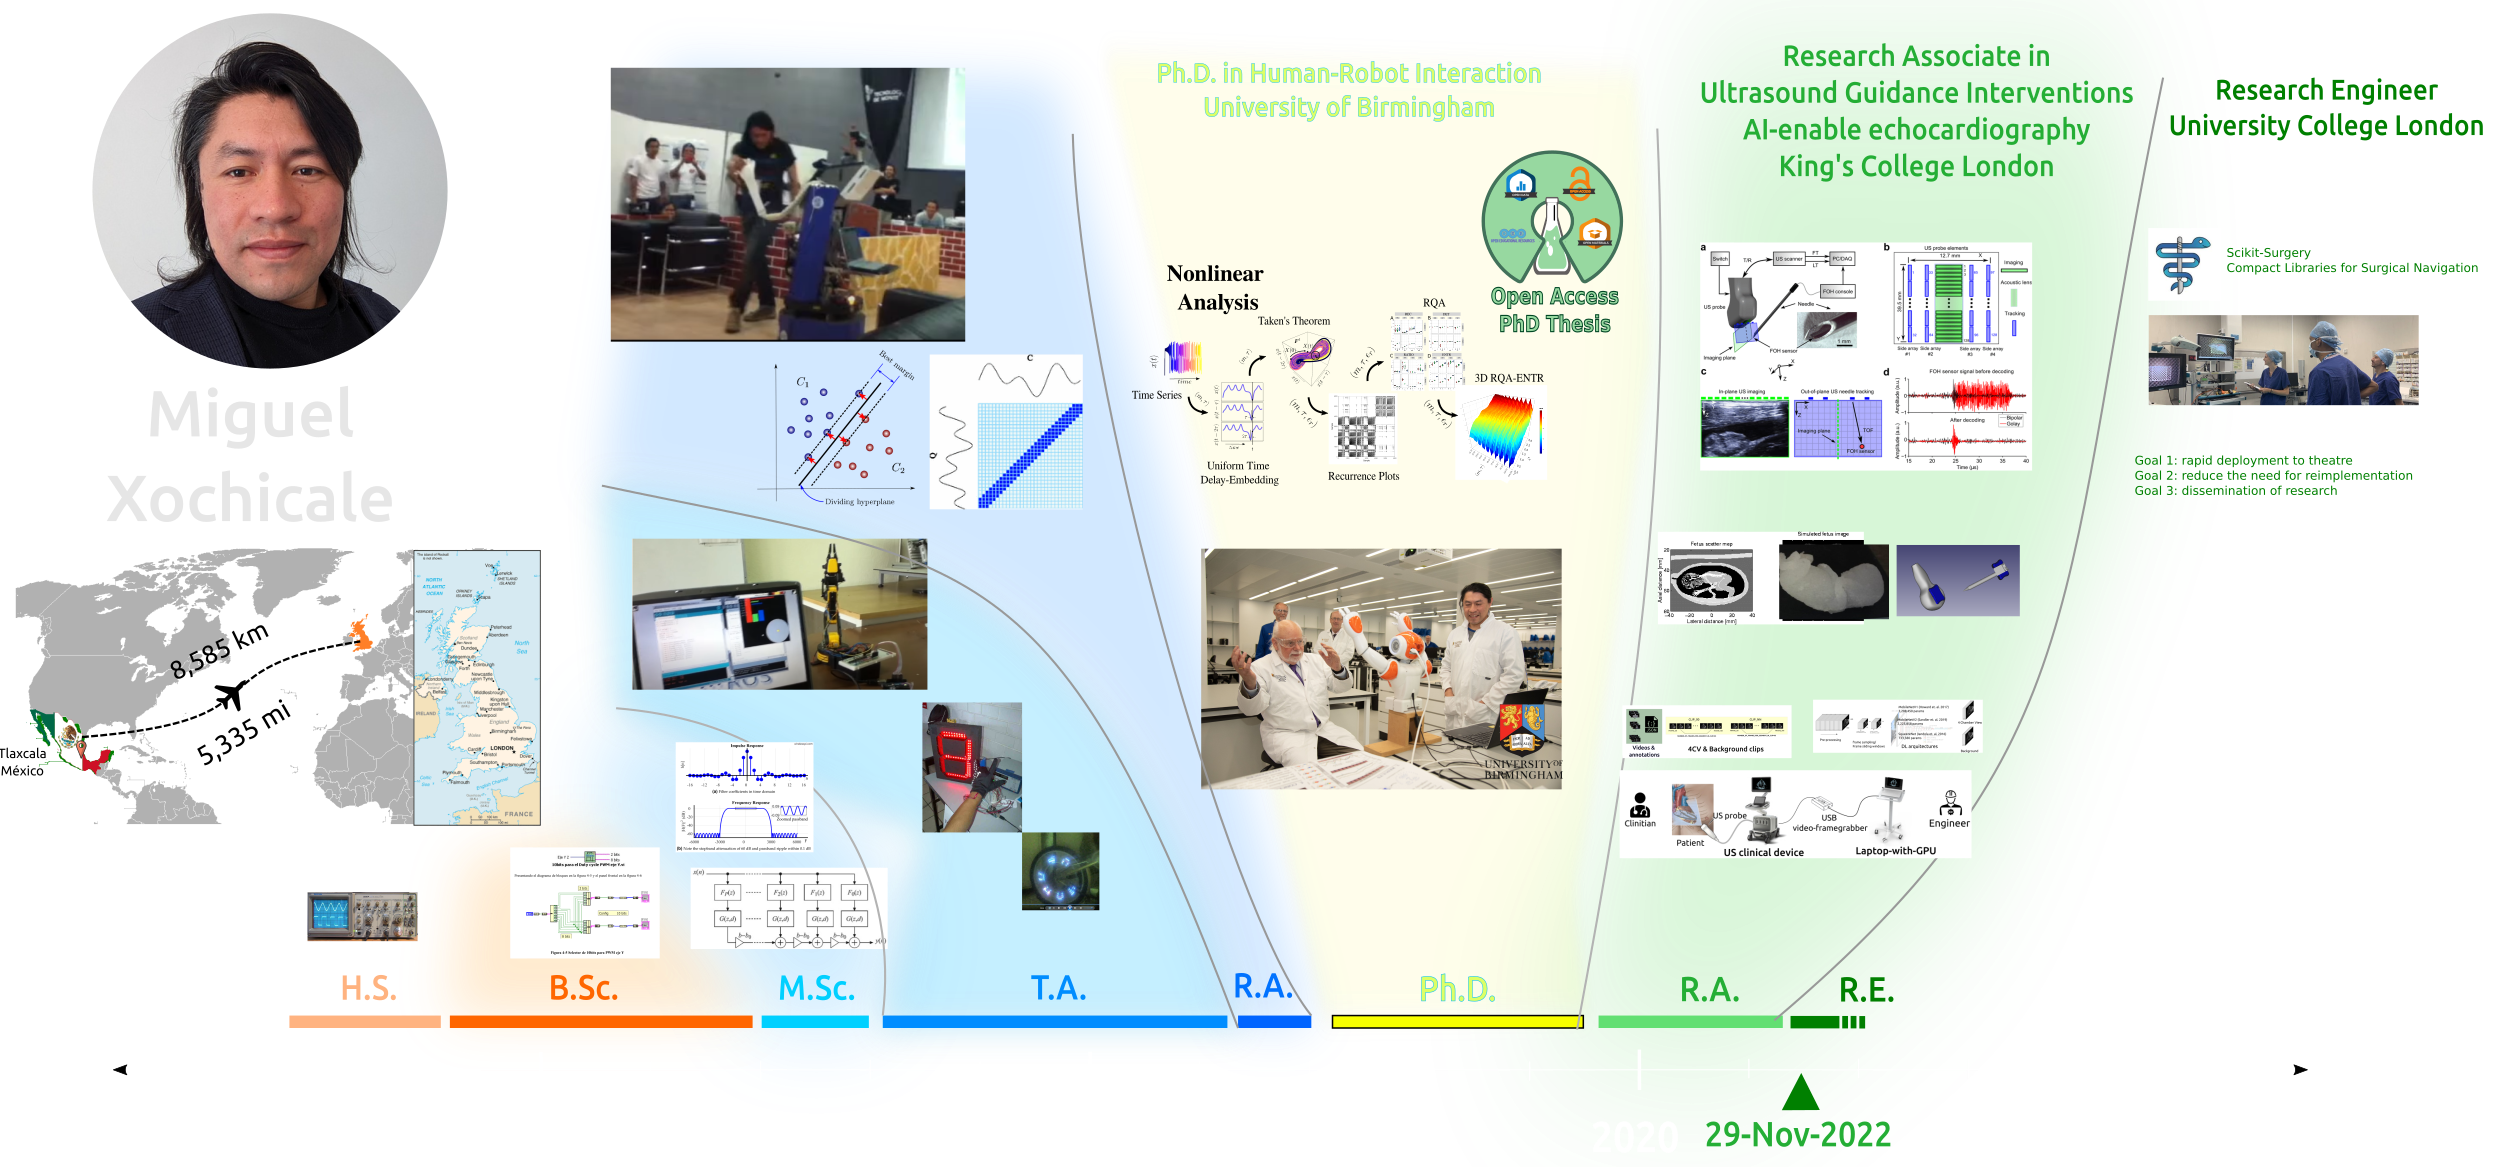
\includegraphics[width=1.0\textwidth]{us-images-of-3d-printed-fetuses/versions/drawing-v05}
        %\caption{}
      \end{figure}
\end{frame}
}




%%%%%%%%%%%%%%%%%%%%%%%%%%%%%%%%%%%%%%%%%%%%
\subsection{Building AI for Medical Devices}


%%%%%%%%%%%%%%%%%%%%%%%%%%%%%%%%%%%%%%%%%%%%%%%%%%%%%%%%
{
%\paper{(a) Coordinate systems overview sketch in 3D Slicer,  (b) Asselin et al. 2018 in conf-BIVPCS, (c) US-simulator, and (d) 3D-printed fetus}
\paper{
Clara AGX: https://www.nvidia.com/en-gb/clara/intelligent-medical-instruments/;
Clara holoscan EGX: https://developer.nvidia.com/clara-holoscan-sdk
}
\begin{frame}{Building AI for Medical Devices}

      \begin{figure}
        \centering
        \includegraphics[width=1.0\textwidth]{medical-devices/versions/drawing-v01}
      \end{figure}


\end{frame}
}



% %%%%%%%%%%%%%%%%%%%%%%%%%%%%%%%%%%%%%%%%%%%%
% \subsection{Potential outcomes}

% %%%%%%%%%%%%%%%%%%%%%%%%%%%%%%%%%%%%%%%%%%%%%%%%%%%%%%%%
% {
% %\paper{(a) Coordinate systems overview sketch in 3D Slicer,  (b) Asselin et al. 2018 in conf-BIVPCS, (c) US-simulator, and (d) 3D-printed fetus}
% %\paper{}
% \begin{frame}{Potential outcomes}


%       \begin{figure}
%         \centering
%         \includegraphics[width=1.0\textwidth]{potential-outcomes/versions/drawing-v00.png}
%       \end{figure}


% \end{frame}
% }





% %%%%%%%%%%%%%%%%%%%%%%%%%%%%%%%%%%%%%%%%%%%%%%%%%%%%%%%%
% {
% %\paper{Wright-Gilbertson M. 2014 in PhD thesis}
% \begin{frame}{Research Questions}	
%  %Can we understand more about fetal development trough the development of more realistic phantoms
% %Can dynamic fetal phantoms be created to understand fetal development?  %added Thu 15 Apr 05:20:09 BST 2021
% %Can synthetic fetus help to understand fetal development? %Fri 23 Apr 05:56:53 BST 2021
% %* Can the creation of synthetic fetuses help to understand fetal development? %Wed 12 May 08:20:58 BST 2021 
% %* Can the creation of synthetic fetuses predict fetal development issues? %Wed 12 May 09:50:47 BST 2021

% \BigSizeFont
% \begin{itemize}
% %\item Would the creation of synthetic fetuses help to understand 
% %the biomechatincs of phetal development? %Sat 15 May 14:51:42 BST 2021
% %\item Can we understand fetal development with synthetic fetuses? %Sat 15 May 15:08:19 BST 2021
% %\item Can the understanding of fetal biomechanics lead to predict fetal pathologies? %Mon 12 Jul 09:25:41 BST 2021
% % MORE ON FETAL PATHOLOGIES:https://www.sciencedirect.com/topics/medicine-and-dentistry/fetal-pathology
% \item Can fetal biomechanics help to understand the prediction of fetal pathologies? %% Mon 12/07/2021 09:45
% \item Would AI-based fetal biomechanics automatically predict fetal pathologies? %Tue 19 Oct 16:54:45 BST 2021
% \item \end{itemize}

% \end{frame}
% }



% %%%%%%%%%%%%%%%%%%%%%%%%%%%%%%%%%%%%%%%%%%%%%%%%%%%%%%%%
% {
% %\paper{Wright-Gilbertson M. 2014 in PhD thesis}
% \begin{frame}{Research Questions}	
%  %Can we understand more about fetal development trough the development of more realistic phantoms
% %Can dynamic fetal phantoms be created to understand fetal development?  %added Thu 15 Apr 05:20:09 BST 2021
% %Can synthetic fetus help to understand fetal development? %Fri 23 Apr 05:56:53 BST 2021
% %* Can the creation of synthetic fetuses help to understand fetal development? %Wed 12 May 08:20:58 BST 2021 
% %* Can the creation of synthetic fetuses predict fetal development issues? %Wed 12 May 09:50:47 BST 2021

% \BigSizeFont
% \begin{itemize}
% %\item Would the creation of synthetic fetuses help to understand 
% %the biomechatincs of phetal development? %Sat 15 May 14:51:42 BST 2021
% %\item Can we understand fetal development with synthetic fetuses? %Sat 15 May 15:08:19 BST 2021
% %\item Can the understanding of fetal biomechanics lead to predict fetal pathologies? %Mon 12 Jul 09:25:41 BST 2021
% % MORE ON FETAL PATHOLOGIES:https://www.sciencedirect.com/topics/medicine-and-dentistry/fetal-pathology
% % \item Can fetal biomechanics help to understand the prediction of fetal pathologies? %% Mon 12/07/2021 09:45
% % \item Would AI-based fetal biomechanics automatically predict fetal pathologies? %Tue 19 Oct 16:54:45 BST 2021

% \item Can GAN-based approaches help to address the scarcity of non-available datasets?
% \item How can AI-based algorthims be less user-dependant and machine-dependant?
% \end{itemize}

% \end{frame}
% }




